\newpage
%**************************************************************
% CAPITOLO 3
%**************************************************************

\chapter{Il progetto di e-commerce VR}
\label{cap:ilprogettoe-commercevr}

\section{Pianificazione del lavoro}

In questa sezione tratterò della pianificazione del lavoro effettuata assieme al mio tutor, delle fasi che l'hanno caratterizzata e del ciclo di vita adottato. 

\section{Ricerca e sperimentazione}

In questa sezione descriverò la fase di ricerca e sperimentazione delle tecnologie utilizzate, inizialmente a me sconosciute. Ho deciso di dedicare una sezione a questa fase perché ha avuto una rilevante importanza all'interno del mio stage e rappresenta uno dei principali obbiettivi aziendali.

\section{Tecnologie adottate}

In questa sezione descriverò come le ricerche e le sperimentazioni effettuate mi hanno portato a scegliere un particolare stack tecnologico.

\section{Analisi dei requisiti}

Questa sezione tratta dei casi d'uso e dei requisiti che il \textit{team} ha ricavato durante la discussione nella prima riunione di stage. Tale analisi ha subito un sostanzioso cambiamento durante la settimana 6, settimana dedicata alla prototipazione del possibile processo d'acquisto all'interno dell'ambiente virtuale. A causa della sua scarsa usabilità, abbiamo deciso di non utilizzare una tastiera virtuale all'interno dell'ambiente tridimensionale per dare la possibilità all'utente di immettere i propri dati e gli estremi di pagamento. Ciò ha portato il \textit{team} a prevedere una registrazione al normale sito di \textit{e-commerce} prima dell'utilizzo dell'app, dove dar la possibilità all'utente di immettere i dati di pagamento. La sezione 3.5.2 spiega in maniera approfondita le sperimentazioni e le discussioni effettuate che hanno portato a questa importante decisione. 


\subsection{Caratteristiche degli utenti}

Obbligare l'utente ad immettere dati sensibili e strettamente personali, come gli estremi di pagamento, prima dell'effettivo utilizzo del servizio non è una buona prassi. L'utente che si appresta per la prima volta ad utilizzare l'applicazione, potrebbe non conoscere l'azienda di produzione e potrebbe non fidarsi. Dunque sono stati delineati due principali tipologie d'utente:

\begin{itemize}
	\item \textbf{Utente registrato visitatore:} utente che ha effettuato la registrazione ma che ha deciso di non immettere i propri dati della carta di credito. Ad esso è permesso visualizzare l'ambiente \textit{VR}\ped{\hyperlink{vr}{G}}, selezionare i prodotti e conoscerne le caratteristiche, aggiungerli al carrello, che sarà reso persistente, ma non di concluderne l'acquisto;
	\item \textbf{Utente registrato acquirente:} utente che ha effettuato la registrazione immettendo anche i dati della carta di credito. Ad esso è permessa la totale esperienza incluso l'acquisto dei prodotti presenti nel carrello.
\end{itemize}

\label{Gerarchia utenti}
\begin{figure}[ht]
	\begin{center}
		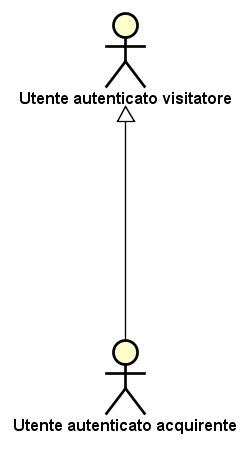
\includegraphics[scale=0.8]{utenti}
		\caption{Gerarchia degli utenti}
	\end{center}
\end{figure}
\FloatBarrier

\subsection{Casi d'uso}

Verranno di seguito elencati tutti i casi d'uso individuati dal \textit{team} per l'applicazione, che spiegano in che modo un utente possa interagire con l'applicazione. Per ogni caso d'uso viene mostrato uno schema \hyperlink{uml}{UML} che ne rappresenta il flusso operativo. \\ Non vengono considerati i casi d'uso relativi alla registrazione al sito/e-commerce poiché tale funzionalità non è stata da me implementata non essendo di mia competenza.

\subsubsection{Caso d'uso UC1: Autenticazione}

\begin{itemize}
	\item \textbf{Attori:} utente registrato visitatore, utente registrato acquirente;
	\item \textbf{Descrizione:} l'utente viene invitato ad immettere l'\textit{username} e la \textit{passowrd} scelti in fase di registrazione;
	\item \textbf{Precondizione:} l'applicazione è avviata e mostra la pagina di login;
	\item \textbf{Postcondizione:} l'autenticazione è andata a buon fine e l'applicazione passa in modalità \textit{VR}\ped{\hyperlink{vr}{G}}.
	\item \textbf{Scenario principale:}
	\begin{enumerate}
		\item L'utente può inserire l'\textit{username} (UC1.1);
		\item L'utente può inserire la \textit{passowrd} (UC1.2);
		\item L'utente può confermare i dati inseriti premendo sul pulsante di login (UC1.3).
	\end{enumerate}
	\item \textbf{Estensioni:} L'utente può visualizzare un messaggio di errore se i dati immessi non corrispondono a quelli di registrazione o se il campo \textit{username} e \textit{passowrd} sono vuoti (UC1.4).
\end{itemize}

\label{UC1}
\begin{figure}[ht]
	\begin{center}
		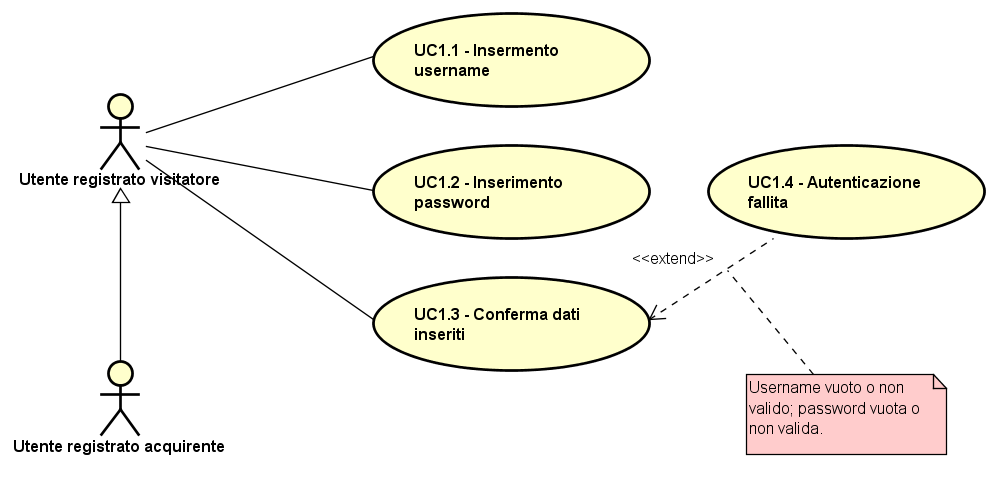
\includegraphics[scale=0.55]{usecase/uc1}
		\caption{UC1: Autenticazione}
	\end{center}
\end{figure}
\FloatBarrier

\subsubsection{Caso d'uso UC2: Interazione con l'ambiente virtuale}

\begin{itemize}
	\item \textbf{Attori:} utente registrato visitatore, utente registrato acquirente;
	\item \textbf{Descrizione:} l'utente, collegato il telefono al visore e indossato quest'ultimo, si ritrova ad osservare un ambiente virtuale con il quale può interagire;
	\item \textbf{Precondizione:} l'utente ha effettuato con successo l'autenticazione;
	\item \textbf{Postcondizione:} l'utente interagisce con l'ambiente virtuale e se è acquirente può comprare gli oggetti presenti nel carrello;
	\item \textbf{Scenario principale:}
	\begin{enumerate}
		\item L'utente può interagire con un oggetto, segnalato da un apposito simbolo, presente nell'ambiente virtuale (UC2.1);
		\item L'utente può interagire con il carrello presente nell'ambiente e segnalato da un'apposita scritta (UC2.2);
		\item L'utente può uscire dall'applicazione effettuando così il logout (UC2.3).
	\end{enumerate}
\end{itemize}

\label{UC2}
\begin{figure}[ht]
	\begin{center}
		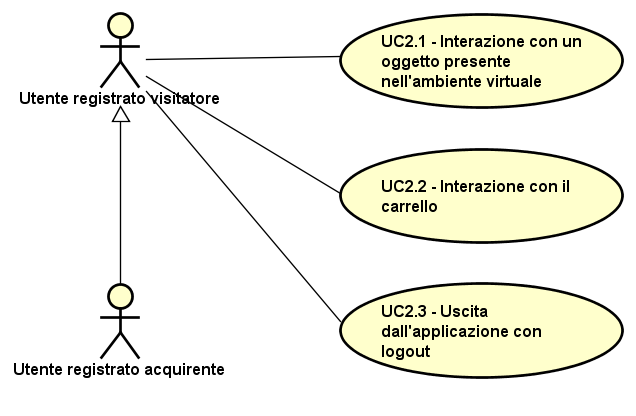
\includegraphics[scale=0.7]{usecase/uc2}
		\caption{UC2: Interazione con l'ambiente virtuale}
	\end{center}
\end{figure}
\FloatBarrier

\subsubsection{Caso d'uso UC2.1: Interazione con un oggetto}

\begin{itemize}
	\item \textbf{Attori:} utente registrato visitatore, utente registrato acquirente;
	\item \textbf{Descrizione:} l'utente interagisce con un oggetto presente nell'ambiente tramite l'interfaccia fisica del visore, attivando il pannello informativo. All'interno di questo sono riportate tutte le informazioni del prodotto e le sue foto. Da pannello è possibile aggiungere l'oggetto al carrello;
	\item \textbf{Precondizione:} l'utente ha effettuato con successo l'autenticazione;
	\item \textbf{Postcondizione:} l'utente interagisce con l'oggetto attivando il pannello informativo.
	\item \textbf{Scenario principale:}
	\begin{enumerate}
		\item Visualizzazione informazioni dell'oggetto sul pannello informativo (UC2.1.1);
		\item Scorrimento foto dell'oggetto sul pannello informativo (UC2.1.2);
		\item Aggiunta oggetto al carrello selezionando l'apposito pulsante (UC2.1.3).
	\end{enumerate}
\end{itemize}

\label{UC2.1}
\begin{figure}[ht]
	\begin{center}
		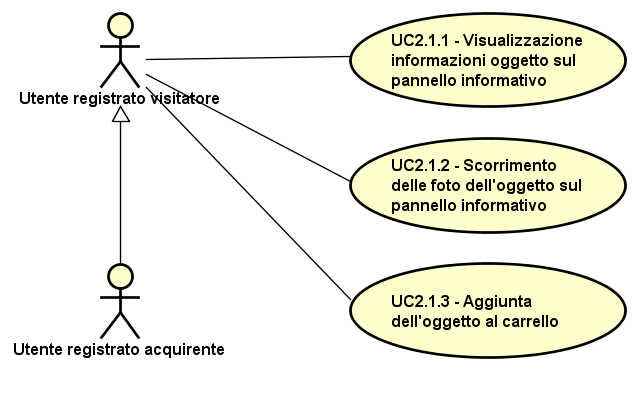
\includegraphics[scale=0.7]{usecase/uc2_1}
		\caption{UC2.1: Interazione con un oggetto}
	\end{center}
\end{figure}
\FloatBarrier

\subsubsection{Caso d'uso UC2.2: Interazione con il carrello}

\begin{itemize}
	\item \textbf{Attori:} utente registrato visitatore, utente registrato acquirente;
	\item \textbf{Descrizione:} entrambe le tipologie possono interagire con il carrello segnalato nell'ambiente da un'apposita scritta. All'interno di esso sono visibili gli oggetti precedentemente inseriti. E' possibile, attraverso l'interfaccia fisica del visore, eliminarli uno ad uno o svuotare completamente il carrello. Se l'utente registrati è acquirente allora può procedere al pagamento;
	\item \textbf{Precondizione:} l'utente ha effettuato l'autenticazione;
	\item \textbf{Postcondizione:} l'utente visualizza i prodotti presenti nel carrello, potendoli acquistare se è acquirente;
	\item \textbf{Scenario principale:}
	\begin{enumerate}
		\item L'utente visualizza il pannello tridimensionale che rappresenta il carrello dove sono elencati i prodotti aggiunti precedentemente (UC2.2.1);
		\item L'utente può eliminare singolarmente un oggetto dal carrello (UC2.2.2);
		\item L'utente può svuotare completamente il carrello (UC2.2.3);
		\item Se l'utente è acquirente allora può procedere con l'acquisto dei prodotti (UC2.2.4);
	\end{enumerate}
\end{itemize}

\label{UC2.2}
\begin{figure}[ht]
	\begin{center}
		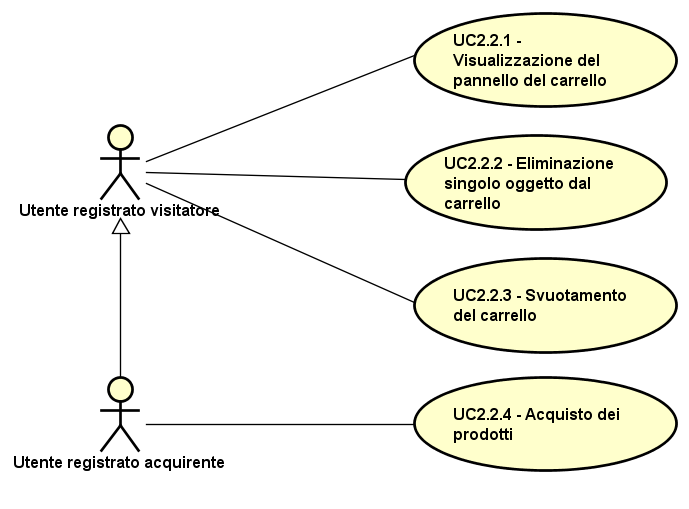
\includegraphics[scale=0.7]{usecase/uc2_2}
		\caption{UC2.2: Interazione con il carrello}
	\end{center}
\end{figure}
\FloatBarrier

\subsection{Requisiti}

Vengono di seguito elencati tutti i requisiti funzionali che l'applicazione deve soddisfare in base ai casi d'uso trovati. Un requisito funzionale rappresenta una \textit{feature} che l'applicazione deve mettere a disposizione all'utente per garantirgli un'esperienza completa. \\
Ogni requisito funzionale è rappresentato da un codice identificativo RFx e da una descrizione che ne illustra lo scopo.

\begin{table}
	\centering
	\label{my-label}
	\begin{tabular}{| l | p{10cm} |}
		\hline
		Requisito & Descrizione \\ \hline
		RF1 & L'applicazione deve permettere all'utente di potersi autenticare utilizzando \textit{username} e \textit{password} specificati in fase di registrazione \\ \hline
		RF1.1 & L'applicazione deve permettere all'utente di inserire l'\textit{username} \\ \hline
		RF1.2 & L'applicazione deve permettere all'utente di inserire la \textit{password} \\ \hline
		RF1.3 & L'applicazione deve permettere all'utente di confermare i dati di autenticazione ed effettuare così il login \\ \hline
		RF2 & L'applicazione deve permettere all'utente di visualizzare l'ambiente virtuale una volta indossato il visore e di interagire con esso \\ \hline
		RF2.1 & L'applicazione deve permettere all'utente di interagire con un oggetto presente nella scena attraverso l'interfaccia fisica offerta dal visore \\ \hline
		RF2.1.1 & L'applicazione deve visualizzare le informazioni relative all'oggetto selezionato all'interno di un panello informativo posto davanti all'utente \\ \hline
		RF2.1.2 & L'applicazione deve permettere la visualizzazione e lo scorrimento delle foto dell'oggetto selezionato all'interno del pannello informativo \\ \hline
		RF2.1.3 & L'applicazione deve permettere l'aggiunta al carrello dell'oggetto selezionato \\ \hline
		RF2.2 & L'applicazione deve permettere l'interazione col carrello segnalato da un'apposita scritta all'interno dell'ambiente virtuale \\ \hline
		RF2.2.1 & L'applicazione deve visualizzare tutti gli oggetti presenti nel carrello precedentemente aggiunti \\ \hline
		RF2.2.2 & L'applicazione deve permettere all'utente di eliminare un singolo oggetto dal carrello \\ \hline
		RF2.2.3 & L'applicazione deve permettere di svuotare completamente il carrello \\ \hline
		RF2.2.4 & L'applicazione deve permettere l'acquisto dei prodotti se l'utente è registrato acquirente \\ 
		\hline
	\end{tabular}
	\caption{Tabella dei requisiti funzionali che l'applicazione deve soddisfare}
\end{table}
\FloatBarrier

\section{Progettazione}

Questa sezione descrive le più importanti e peculiari fasi di progettazione dell'applicazione. Molte delle decisioni prese sono state discusse da me assieme al \textit{team} di The White Dog s.r.l., cercando il più possibile di accontentare gli \textit{stakeholder}\hyperlink{sh}{\ped{G}}, ovvero il signor Stefano Mocellini, fondatore dell'azienda, attraverso l'ancora giovane e incompleta tecnologia \textit{VR}\ped{\hyperlink{vr}{G}}.

\subsection{Portabilità dell'applicazione}

Una delle sfide più impegnative di questo progetto era riuscire a sviluppare l'applicazione per entrambi i dispositivi: \textit{Samsung Gear VR} e \textit{Google Cardboard}. Prima di conoscere a basso livello tali tecnologie, avevamo progettato l'implementazione di un'interfaccia che riconoscesse la tecnologia in uso e che ne richiamasse così i metodi specifici. Purtroppo, dopo aver sperimentato gli \textit{SDK}\ped{\hyperlink{sdk}{G}} forniti da entrambe le piattaforme e seguito i due principali tutorial\footnote[1]{\textit{Samsung Gear VR:} \url{http://www.samsung.com/us/samsungdeveloperconnection/developer-resources/gear-vr.html} \\ \textit{Google Cardboard:} \url{https://developers.google.com/vr/unity/}}, mi sono reso conto che una totale portabilità non era possibile a causa delle forti differenze tra le due piattaforme. \\ \\
La prima differenza, e la più importante, è la \textbf{MainCamera} o Camera Principale. In un progetto \textit{Unity}, ogni scena possiede una o più camere che rappresentano il punto di vista dell'utente. Una camera normale non permette l'esperienza \textit{VR}\ped{\hyperlink{vr}{G}} poiché non è collegata ai sensori di movimento e rotazione del dispositivo. All'interno dei pacchetti \textit{Unity} offerti agli sviluppatori dalle due case, sono presenti le rispettive camere \textit{VR}\ped{\hyperlink{vr}{G}} che, tramite script ad esse agganciati, permettono l'esperienza \textit{VR}\ped{\hyperlink{vr}{G}} una volta posizionate a piacimento all'interno della scena. Tali script si collegano direttamente ai sensori del dispositivo che è diverso per le due piattaforme. Il visore \textit{Samsung Gear VR} possiede al suo interno tutti i sensori di movimento e rotazione necessari e lo script, agganciato alla \textit{MainCamera}, legge i dati derivanti da essi. Invece, i dispositivi \textit{Google Cardboard} non possiedono alcun sensore e la \textit{MainCamera} legge i dati di rotazione e movimento dai sensori all'interno dello \textit{smartphone}. Questa profonda differenza hardware causa una forte differenza tra i due script della \textit{MainCamera}, obbligando ad inserire due camere diverse all'interno della stessa scena.

\label{MainCamera}
\begin{figure}[ht]
	\begin{center}
		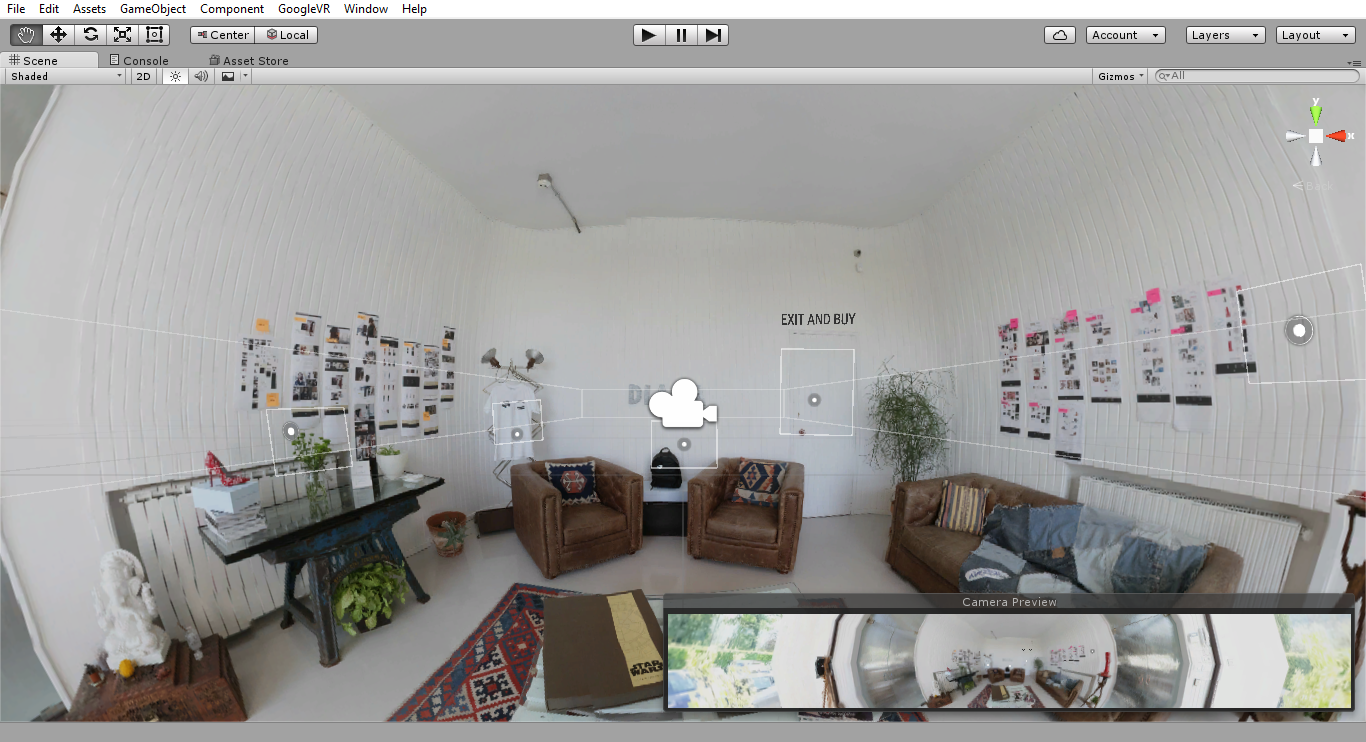
\includegraphics[scale=0.35]{maincamera}
		\caption{Camera VR posizionata all'interno dell'ambiente tridimensionale creato in Unity}
	\end{center}
\end{figure}
\FloatBarrier

La seconda importante differenza è l'implementazione degli \textbf{oggetti interattivi} all'interno della scena \textit{Unity}. Di base, sia per \textit{Samsung Gear VR} sia per \textit{Google Cardboard}, un oggetto per essere interattivo necessità di due caratteristiche:

\begin{itemize}
	\item \textbf{Mesh Collider:} è necessario aggiungere tale proprietà all'oggetto che si vuole rendere interattivo. Tale proprietà rende un oggetto "tangibile", ovvero può essere colliso da un altro oggetto presente nella scena. Questo permette alla \textit{Camera VR} di interagire con l'oggetto inviando un "raggio virtuale" verso quest'ultimo che, scontrandovisi, potrà attivare gli eventi che si desidera;
	\item \textbf{InteractiveScriptVR:} script, da agganciare all'oggetto, che cattura l'evento di selezione attraverso i metodi esposti dall'\textit{api} della particolare piattaforma. All'interno di questi metodi si può implementare il vero comportamento dell'oggetto interattivo.  
\end{itemize}

L'\texttt{InteractiveScriptVR} differisce profondamente da una piattaforma all'altra. \\
Per quanto riguarda \textit{Google Cardboard}, lo script implementa la classe \texttt{IGvrGazeResponder}, la quale espone i metodi per la cattura della selezione tramite lo spostamento del magnete posto lateralmente nel visore. \\
Per quanto riguarda \textit{Samsung Gear VR} invece, l'\textit{InteractiveScriptVR} non implementa alcuna interfaccia ma necessita l'utilizzo del namespace \texttt{VRStandardAsset.Utils} per richiamare i metodi esposti dallo script \texttt{VRInteractiveItem}, script che va agganciato all'oggetto come l'\textit{InteractiveScriptVR}. \\
Questa differenza di implementazione degli oggetti interattivi, rende davvero difficoltosa la loro portabilità da una piattaforma all'altra. Dunque, dopo una lunga discussione avvenuta nell'ufficio R\&D, abbiamo deciso di abbandonare la totale portabilità dell'applicazione, raggiungendo però un compromesso: la separazione della cattura dell'evento di selezione dall'effettivo comportamento dell'oggetto, implementandoli in due script differenti. In questo modo è stato possibile creare dei \textit{prefabs} (oggetti portabili all'interno dell'ambiente \textit{Unity} contenenti le informazioni di forma, colore, script agganciati eccetera) che contenessero solo le informazioni del comportamento dell'oggetto dopo la cattura della selezione, caratteristica assolutamente indipendente dalla piattaforma.    

\subsection{Usabilità dell'applicazione}

La fase di acquisto inizialmente prevista comprendeva l'immissione dei propri dati di pagamento all'interno dell'ambiente \textit{VR}\ped{\hyperlink{vr}{G}} tramite una tastiera tridimensionale posta davanti all'utente, dove ogni tasto era selezionabile attraverso l'interfaccia fisica del visore. Dopo la sperimentazione di tale tastiera, abbiamo constatato la sua scarsa usabilità, causando un processo d'acquisto lungo e tedioso. Abbiamo dunque optato per una soluzione più semplice: l'utente prima di entrare nella scena \textit{VR}\ped{\hyperlink{vr}{G}} viene invitato a immettere i propri dati di login attraverso la normale tastiera del telefono, così da accedere al proprio account personale. Tale account deve essere precedentemente creato nel sito/e-commerce dedicato, dove possono essere immessi anche i dati di pagamento. Una volta autenticato, lo \textit{smartphone} passa in modalità \textit{VR}\ped{\hyperlink{vr}{G}}, invitando l'utente ad indossare il visore. All'interno dell'ambiente, all'utente non viene più richiesto di immettere dati, così da poter sperimentare in tutta serenità l'esperienza \textit{VR}\ped{\hyperlink{vr}{G}}. \\
Questa soluzione però ha mostrato al \textit{team} la profonda differenza tra le piattaforme \textit{Samsung Gear VR} e \textit{Google Cardboard}. Ogni applicazione \textit{Samsung Gear VR}, una volta avviata, richiede all'utente di inserire lo \textit{smartphone} all'interno del visore prima di poter effettivamente essere utilizzata. Questo obbliga lo sviluppatore a prevedere tutte scene di tipo \textit{VR}\ped{\hyperlink{vr}{G}} durante lo sviluppo dell'applicazione, contrariamente a \textit{Google Cardboard} che permette la coesistenza di tutte le tipologie scenografiche: 2D, 3D e \textit{VR}\ped{\hyperlink{vr}{G}}. Dunque, non è stato possibile inserire una scena 2D iniziale di login per la piattaforma Samsung e, a causa dei tempi ridotti di stage, non è stato possibile sviluppare una soluzione a tale problema.

\label{Login}
\begin{figure}[ht]
	\begin{center}
		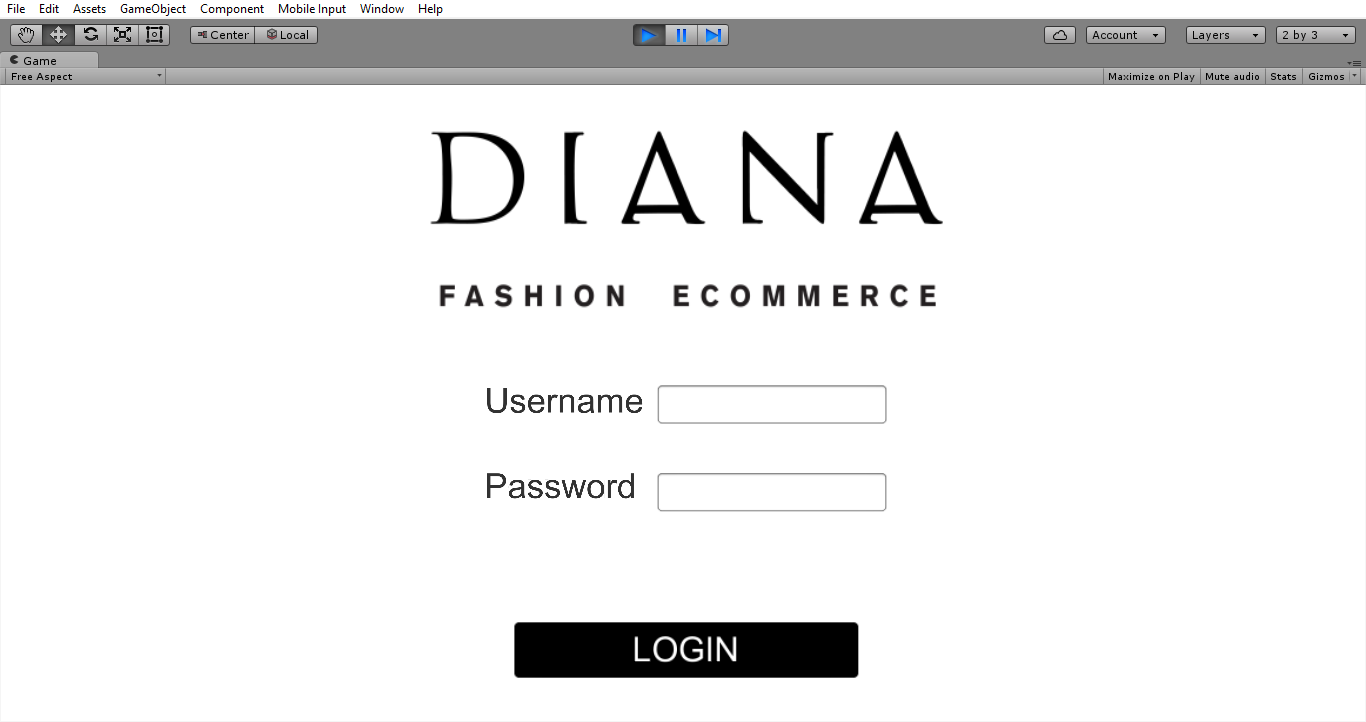
\includegraphics[scale=0.35]{login}
		\caption{Schermata 2D di login}
	\end{center}
\end{figure}
\FloatBarrier

\subsection{Costruzione della scena 3D}

Dopo un'attenta fase di ricerca iniziale sulla tecnologia \textit{Unity} e \textit{VR}\ped{\hyperlink{vr}{G}}, ho potuto constatare che vi sono due modi principali per costruire una scena 3D:

\begin{itemize}
	\item \textbf{Tramite modellazione 3D dell'intero ambiente virtuale};
	\item \textbf{Tramite l'applicazione di una foto a 360 gradi di una stanza ad una sfera o cubo inversi}.
\end{itemize}

La prima soluzione permette una vera esperienza 3D, dando la possibilità all'utente di spostarsi nelle tre dimensioni, prevedendo l'utilizzo di un gamepad. Ogni oggetto è ben definito in un punto nello spazio tridimensionale e osservabile da tutte le angolazioni. Purtroppo però per costruire un ambiente 3D di qualità accettabile sono necessarie profonde conoscenze di modellazione, conoscenze che fuoriescono dall'obbiettivo di questo stage. \\
La seconda soluzione non permette una totale esperienza 3D, poiché applica una foto 2D a 360 gradi ad una sfera o un cubo inversi creati in \textit{Unity}. L'effetto così creato simula la tridimensionalità, non permettendo all'utente lo spostamento tra gli oggetti ma solo una visione stereoscopica della stanza. Il livello qualitativo raggiunto però è ottimo, se la foto viene realizzata con le giuste apparecchiature. Abbiamo deciso dunque di utilizzare la seconda metodologia per la creazione dell'ambiente. \\
Abbiamo così realizzato la foto a 360 gradi utilizzando una macchinetta fotografica di alta qualità presente nell'azienda seguendo la guida presente nel sito \url{...}. Posizionata la macchinetta fotografica al centro di una stanza appositamente arredata allo scopo nell'azienda Diana Corp., abbiamo effettuato 3 foto, una sovraesposta, una sottoesposta e una ad esposizione normale, ogni 45 gradi orizzontalmente. Abbiamo poi ripetuto l'operazione inclinando la macchinetta 45 verso il basso e infine 45 gradi verso l'alto. Le foto così ottenute, ci hanno permesso di creare la foto a 360 gradi tramite il software ..., che l'ha creata automaticamente a meno di qualche punto di agganciamento inserito manualmente. Infine abbiamo applicato la foto come texture di una sfera inversa creata tramite l'editor di \textit{Unity}.

\label{Sfera}
\begin{figure}[ht]
	\begin{center}
		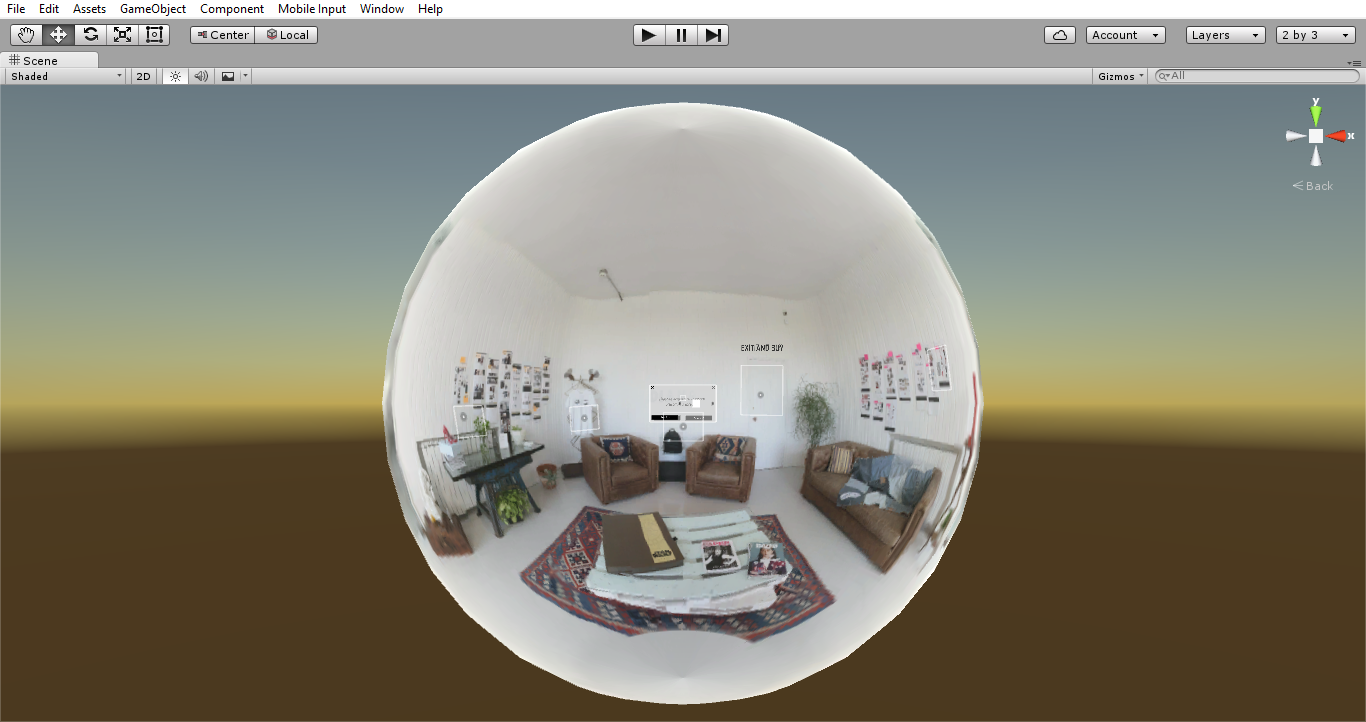
\includegraphics[scale=0.35]{sfera}
		\caption{Sfera inversa a cui è stata applicata la foto 360 della stanza come texture}
	\end{center}
\end{figure}
\FloatBarrier  

\subsection{Interazione con gli oggetti all'interno della scena} 

All'interno di questa sottosezione parlerò della progettazione riguardante le modalità di interazione tra il visore VR e gli oggetti presenti all'interno della scena.

\subsection{Progettazione e integrazione con AWS API Gateway}

All'interno di questa sezione tratterò della progettazione riguardante l'API Mock creata tramite AWS API Gateway e della sua integrazione con l'applicazione.

\section{Sviluppo}

In questa sezione andrò a descrivere in dettaglio lo sviluppo delle più significative e peculiari funzionalità dell'applicazione.

\subsection{Sviluppo degli oggetti interattivi}

In questa sottosezione descriverò come si costruiscono degli oggetti interattivi in Unity per i dispositivi VR.

\subsection{Creazione a runtime di oggetti interattivi}

In questa sottosezione tratterò della creazione a runtime di oggetti interattivi in Unity.

\subsection{Dati persistenti attraverso le scene}

In questa sezione spiegherò come si costruiscono oggetti persistenti che vivono attraverso le scene.

\subsection{Unity e il protocollo HTTP}

In questa sottosezione parlerò di come Unity si integri con il protocollo HTTP.

\subsection{Creazione e parsing di oggetti JSON in Unity}

In questa sottosezione parlerò di come si creino e si manipolino oggetti JSON in Unity.

\section{Verifica e validazione}

All'interno di questa sezione parlerò della fase di verifica e validazione effettuata per questo progetto.
